\documentclass{standalone}

\renewcommand{\familydefault}{\sfdefault}
\usepackage{amsmath}
\usepackage{tikz}
\usetikzlibrary{arrows.meta, positioning, calc, }

\newcommand{\quadrup}[5]{%
  % #1 = x, #2 = y, #3 = largura, #4 = altura, #5 = cor
  \fill[#5]
    (#1-0.5*#3,#2+0.5*#4) --
    (#1,#2) --
    (#1+0.5*#3,#2+0.5*#4) --
    cycle;
  \fill[#5]
    (#1-0.5*#3,#2-0.5*#4) --
    (#1,#2) --
    (#1+0.5*#3,#2-0.5*#4) --
    cycle;
}

\newcommand{\bpmrule}[4]{%
  % #1 = x_inicial, #2 = altura total H, #3 = número de marcas, #4 = cor
  \draw[#4, thick] (#1,-0.5*#2) -- (#1,0.5*#2);
  \foreach \x in {1,...,#3} {
    \pgfmathparse{\x == 33 ? 1 : 0}
    \ifnum\pgfmathresult>0\relax
      \draw[#4, thick] (#1, 0.5*#2 - #2*\x/#3 + 0.5*#2/#3)
                    -- ++(0.2,0) node[right, xshift={-0.25em}] {\footnotesize 0};
    \else
      \pgfmathparse{mod(\x - 3,5) == 0 ? 1 : 0}
      \ifnum\pgfmathresult>0\relax
        \draw[#4, thick] (#1, 0.5*#2 - #2*\x/#3 + 0.5*#2/#3)
                    -- ++(0.2,0);
      \else
        \draw[#4, line width=0.65pt] (#1, 0.5*#2 - #2*\x/#3 + 0.5*#2/#3)
                      -- ++(0.1,0);
      \fi
    \fi
  }
}

\begin{document}

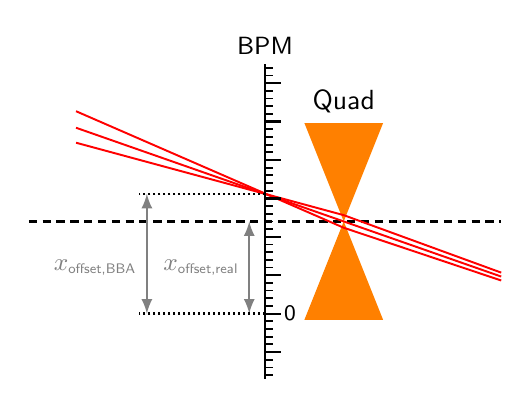
\begin{tikzpicture}[>=latex]
    \coordinate (O) at (0, 0);
    \pgfmathsetmacro{\sbpm}{-1}

    % \coordinate (B) at (\sbpm, 0.7);
    \coordinate (B) at (-2, 0.7);

    \pgfmathsetmacro{\qlarg}{1}   
    \pgfmathsetmacro{\qalt}{2.5}

    \quadrup{0}{0}{\qlarg}{\qalt}{orange}

    \node[above] at ($(O)+(0,\qalt/2)$) {Quad};
    
    \draw[thick, densely dashed] (-4, 0) -- (2, 0);

    % \draw[line width=0.7pt, red, -stealth] ($1.7*(B)$) -- ($-1*(B)$) node[right, yshift={-0.25em}] {\small{beam}};
    \draw[line width=0.7pt, red] ($1.7*(B)$) -- ($-1*(B)$);% node[right, yshift={-0.25em}] {\small{beam}};
    \draw[line width=0.7pt, red] (-3.4, 1.0) -- (0, 0.08) -- (2, -0.65);% node[right, yshift={-0.25em}] {\small{beam}};
    \draw[line width=0.7pt, red] (-3.4, 1.4) -- (0, -0.08) -- (2, -0.75);% node[right, yshift={-0.25em}] {\small{beam}};


    % régua
    \bpmrule{\sbpm}{4}{41}{black}
    \pgfmathsetmacro{\dybba}{-1.17}
    \pgfmathsetmacro{\xbpm}{0.35}
    \node[above, black] at (\sbpm, 2) {\small{BPM}};
    \draw[thick, gray, <->] (\sbpm-0.2, \dybba) -- (\sbpm-0.2, 0) node[midway, left] {\small $x_\text{\tiny{offset,real}}$};
    \draw[thick, gray, <->] (\sbpm-1.5, \dybba) -- (\sbpm-1.5, \xbpm) node[midway, left, yshift={-0.5em}] {\small $x_\text{\tiny{offset,BBA}}$};
    \draw[thick, densely dotted, black] (\sbpm, \xbpm) -- ++(-1.6, 0);
    \draw[thick, densely dotted, black] (\sbpm, \dybba) -- ++(-1.6, 0);

    
\end{tikzpicture}


\end{document}


% \documentclass{standalone}

% \renewcommand{\familydefault}{\sfdefault}
% \usepackage{amsmath}
% \usepackage{tikz}
% \usetikzlibrary{arrows.meta, positioning, calc, }

% \newcommand{\quadrup}[5]{%
%   % #1 = x, #2 = y, #3 = largura, #4 = altura, #5 = cor
%   \fill[#5]
%     (#1-0.5*#3,#2+0.5*#4) --
%     (#1,#2) --
%     (#1+0.5*#3,#2+0.5*#4) --
%     cycle;
%   \fill[#5]
%     (#1-0.5*#3,#2-0.5*#4) --
%     (#1,#2) --
%     (#1+0.5*#3,#2-0.5*#4) --
%     cycle;
% }

% \newcommand{\bpmrule}[4]{%
%   % #1 = x_inicial, #2 = y, #3 = comprimento (cm), #4 = cor
%   \draw[#4, thick] (#1,-#2*0.5) -- (#1,#2*0.5);
%   \foreach \x in {1,...,#3} {
%     \draw[#4, thick] (#1, #2*0.5 - #2*\x/#3 + 0.5*#2/#3) -- ++(0.1,0);
%     % \node[below] at (#1+\x,#2-0.15) {\footnotesize \x};
%   }
% }

% \begin{document}

% \begin{tikzpicture}[>=latex]
%     \coordinate (O) at (0, 0);
%     \coordinate (B) at (-2, 0.7);

%     \pgfmathsetmacro{\qlarg}{1}   
%     \pgfmathsetmacro{\qalt}{2.5}

%     \quadrup{0}{0}{\qlarg}{\qalt}{orange}

%     \node[above] at ($(O)+(0,\qalt/2)$) {Quad};
    
%     \draw[thick, ->] (-4, 0) -- (2, 0) node[right] {$s$};
%     \draw[thick, ->] (-3.8, -1) -- (-3.8, 1.5) node[above] {$x$};

%     \draw[line width=0.7pt, red, -stealth] ($1.7*(B)$) -- ($-1*(B)$) node[right, yshift={-0.25em}] {\small{beam}};

%     % régua
%     \bpmrule{-2}{4}{51}{gray}
%     \node[above, gray] at (-2, 2) {\small{BPM}};
%     \draw[line width=0.7pt, densely dotted, gray] (B) -- ++(-1.8, 0) node[left] {\small $x_\text{\tiny offset}$};
    
% \end{tikzpicture}


% \end{document}
